% 00_home.tex — Landing page
\section*{Welcome}
\addcontentsline{toc}{section}{Welcome}

In any direction you point a microwave receiver in space, you pick up a faint, almost perfectly uniform glow of $2.7\,\mathrm{K}$ photons. This is the cosmic microwave background — light released $380{,}000$ years after the Big Bang, when the universe first became transparent. It is the oldest electromagnetic signal we can detect, and its tiny anisotropies (one part in $10^{5}$ on the sky) are a high-resolution snapshot of the universe long before stars, galaxies, or any of the structure we see today had formed.

\begin{center}
  
\includegraphics[width=0.85\linewidth]{figures/planck_sky.jpg}\\
  \small\textit{Placeholder: Planck 2018 SMICA temperature map, downloadable from the Planck Legacy Archive. The variations are $\pm 300\,\mu\mathrm{K}$ around the $2.7\,\mathrm{K}$ mean.}
\end{center}

A tutorial about the CMB is really a tutorial about cosmological perturbation theory: how to predict, from a small number of cosmological parameters, the statistical properties of those temperature variations and their polarization counterpart. The aim of this series is to walk through that calculation end-to-end, building a small computational pipeline as we go.

\paragraph{How to use this tutorial.}
Open a Jupyter notebook next to this text. Every code block in the chapters can be pasted directly into a cell and run. By the end you will have computed temperature and polarization spectra from scratch, included gravitational lensing, included primordial gravitational waves, and compared the result against CAMB. The prerequisites chapter walks you through the one-time setup.

\section*{A brief history}
\addcontentsline{toc}{section}{A brief history}

The theoretical prediction came first. In 1948 \emph{Ralph Alpher} and \emph{Robert Herman}, students of \emph{George Gamow}, estimated that the hot early universe should have left behind a relic radiation field at a temperature of a few kelvin. Their paper was largely forgotten. In 1964 \emph{Arno Penzias} and \emph{Robert Wilson} were trying to use a horn antenna at Bell Labs to map radio sources in the Milky Way and could not get rid of a persistent isotropic noise at about $3\,\mathrm{K}$. They were unaware of the prediction. A team at Princeton — \emph{Robert Dicke}, \emph{Jim Peebles}, \emph{David Wilkinson}, and \emph{Peter Roll} — was, independently, building a detector to look for it. When the two groups met, the identification was immediate, and Penzias and Wilson received the 1978 Nobel Prize.

The theoretical machinery for predicting the anisotropies followed in parallel. \emph{Rainer Sachs} and \emph{Arthur Wolfe} (1967) worked out the gravitational redshift contribution that bears their names. \emph{Joseph Silk} (1968) computed the diffusion damping that suppresses small-scale structure. \emph{Rashid Sunyaev} and \emph{Yakov Zel'dovich} (1970) worked out the acoustic peak pattern that we now use to measure the geometry of the universe, as well as the spectral distortions from hot electrons that bear their names. \emph{Wayne Hu} and collaborators in the 1990s built much of the modern framework relating the spectra to cosmological parameters. \emph{Uros Seljak} and \emph{Matias Zaldarriaga} (1996) wrote down the line-of-sight integration method that made the computation tractable; every modern Boltzmann code, including the one in this tutorial, uses it.

Experimentally, the path went COBE (1992, the first anisotropy detection), BOOMERanG and MAXIMA (1998-2000, the first acoustic peaks), WMAP (2003-2010, precision cosmology), Planck (2009-2018, the current gold standard), and ground-based polarization experiments — ACT, SPT, BICEP/Keck — that are now the most sensitive on small angular scales and on $B$-mode polarization. The next generation, Simons Observatory, CMB-S4, and the LiteBIRD satellite, target the primordial gravitational-wave signature predicted by inflation.

\section*{A short history of the universe}
\addcontentsline{toc}{section}{A short history of the universe}

Times are measured from the Big Bang, in the standard $\Lambda$CDM cosmology with Planck~2018 parameters.

\begin{itemize}[leftmargin=*]
  \item \textbf{$t < 10^{-32}\,\mathrm{s}$ — Inflation.}
    A brief epoch of accelerated, near-de~Sitter expansion. Quantum fluctuations of a light scalar field are stretched to super-horizon scales and frozen in as classical curvature perturbations $\mathcal{R}(\vec{k})$ with a nearly scale-invariant spectrum,
    \[
      \mathcal{P}_{\mathcal{R}}(k) = A_s \left(\frac{k}{k_*}\right)^{n_s - 1}.
    \]
    Tensor modes (gravitational waves) are produced at the same time, with amplitude $A_t = r\, A_s$.

  \item \textbf{$t \sim 10^{-32}$ to $10^{-12}\,\mathrm{s}$ — Reheating, baryogenesis, electroweak transition.}
    The inflaton decays into a hot relativistic plasma. The matter-antimatter asymmetry is generated. The Higgs field condenses; particles become massive.

  \item \textbf{$t \sim 1\,\mathrm{s}$, $T \sim 1\,\mathrm{MeV}$ — Neutrino decoupling.}
    Neutrinos stop interacting with the plasma and free-stream from this point on. Their anisotropic stress is imprinted on the gravitational potentials and observable through a phase shift in the CMB acoustic peaks.

  \item \textbf{$t \sim 3\,\mathrm{min}$ — Big Bang nucleosynthesis.}
    Light element abundances are set by competition between weak rates and the expansion. This fixes the baryon density, independent of the CMB.

  \item \textbf{$t \sim 5\times 10^{4}\,\mathrm{yr}$, $z \sim 3400$ — Matter-radiation equality.}
    Matter density catches up with radiation density. The transition leaves an imprint on the matter power spectrum turnover and on the CMB acoustic peak heights.

  \item \textbf{$t \sim 3.8 \times 10^{5}\,\mathrm{yr}$, $z \sim 1100$ — Recombination.}
    Free electrons and protons combine into neutral hydrogen. Photons last-scatter around this redshift and have travelled freely ever since. \emph{This snapshot is the CMB.}

  \item \textbf{$t \sim 10^{8}$ to $10^{9}\,\mathrm{yr}$, $z \sim 6$-$30$ — Reionization.}
    The first stars and quasars produce UV radiation that re-ionizes intergalactic hydrogen. CMB photons see a second, lower-amplitude scattering surface.

  \item \textbf{$t \sim 10^{9}$ to $1.4\times 10^{10}\,\mathrm{yr}$ — Structure formation and lensing.}
    Matter perturbations grow into halos and the cosmic web. Gradients of the gravitational potential along the line of sight deflect CMB photons by $\sim 2'$, smoothing the acoustic peaks and converting $E$-mode power into a small $B$-mode signal.

  \item \textbf{$t \sim 10^{10}\,\mathrm{yr}$ — Dark energy domination.}
    The universe enters a second period of accelerated expansion. Gravitational potentials decay along the line of sight, producing the late-time integrated Sachs-Wolfe effect on the largest scales.
\end{itemize}

\section*{Why we predict spectra, not maps}
\addcontentsline{toc}{section}{Why we predict spectra, not maps}

The universe is one realization of a stochastic process. We have only one sky, and we cannot rerun the Big Bang. What inflation gives us is a probability distribution over initial conditions: the primordial perturbation $\mathcal{R}(\vec{k})$ is, to excellent approximation, a Gaussian random field. Linear physics turns it into another Gaussian random field, the CMB temperature anisotropy $T(\hat{n})$. \emph{All the information} a Gaussian random field carries is in its two-point function.

The temperature field decomposes on the sphere:
\[
  T(\hat{n}) = \sum_{\ell m} a_{\ell m}\, Y_{\ell m}(\hat{n}),
  \qquad
  \langle a_{\ell m} a^*_{\ell' m'} \rangle = \delta_{\ell\ell'} \delta_{m m'}\, C_\ell.
\]
The angular power spectrum $C_\ell$ is the variance of the $a_{\ell m}$. It is what theory predicts. The map you draw from $\{a_{\ell m}\}$ is one realization; the spectrum is the statistical envelope, and that is what we compare to.

\begin{aside}[Variance of a variance]
A Gaussian random variable $x$ with variance $\sigma^2 = \langle x^2 \rangle$ has zero higher cumulants — the variance fully specifies the distribution. The same is true field-theoretically: a Gaussian random field on the sphere is fully specified by $C_\ell$. ``Spectrum'' here means \emph{variance per multipole}: $C_\ell$ is the expected value of $|a_{\ell m}|^2$ averaged over realizations of the universe. We can only \emph{estimate} this expectation from the $2\ell+1$ available $m$ values at each $\ell$, leading to the irreducible cosmic-variance uncertainty $\Delta C_\ell / C_\ell = \sqrt{2/(2\ell+1)}$ at low $\ell$.
\end{aside}

\section*{Reading the TT spectrum}
\addcontentsline{toc}{section}{Reading the TT spectrum}

The most familiar CMB spectrum is $\mathcal{D}_\ell^{TT} \equiv \ell(\ell+1)C_\ell^{TT}/(2\pi)$ versus $\ell$. It is the central object of this tutorial: by the end of the power-spectrum chapter, the code you wrote will produce it. Below is the prediction from Planck-2018 $\Lambda$CDM, annotated with the physics behind each feature.

\begin{center}
  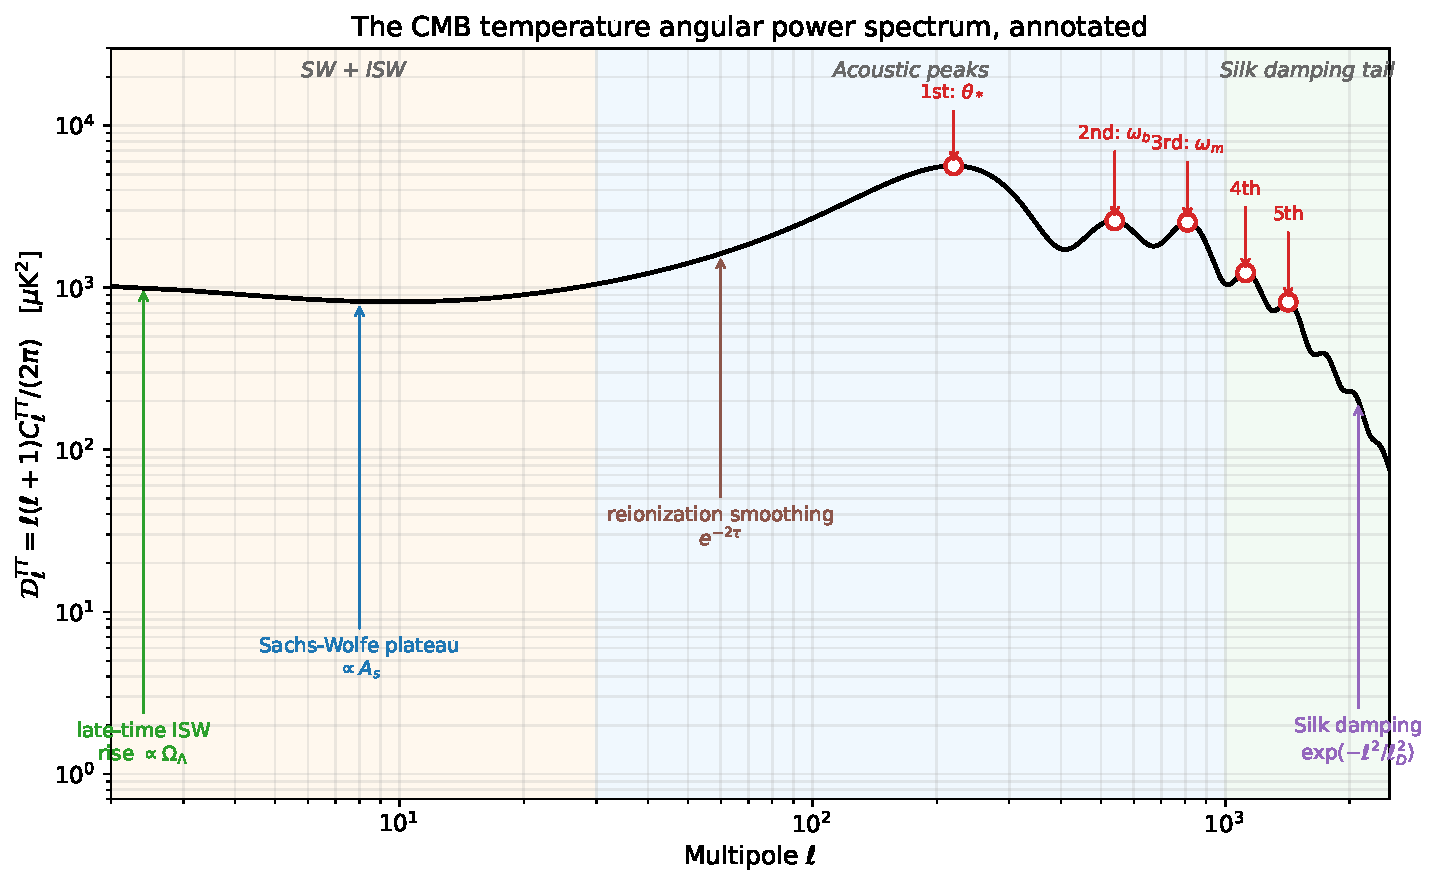
\includegraphics[width=\linewidth]{figures/00_TT_annotated.pdf}
\end{center}

Working through the features:

\begin{itemize}[leftmargin=*]
  \item \textbf{Sachs-Wolfe plateau ($\ell \lesssim 30$).}
    Photons climbing out of large potential wells at last scattering are gravitationally redshifted; this temperature shift is the original Sachs-Wolfe effect. The plateau scales with the primordial amplitude $A_s$ and the gravitational potential normalization.

  \item \textbf{Integrated Sachs-Wolfe rise at the very lowest $\ell$.}
    When a photon transits a time-varying potential along the line of sight it picks up an extra blue/redshift, $\delta T/T = 2\int\dot\Psi_W\,\mathrm{d}\tau$. The potentials decay at late times under dark energy and slightly during the radiation-to-matter transition. The late-time ISW contribution shifts the lowest few multipoles upward; removing dark energy would remove this rise.

  \item \textbf{First acoustic peak at $\ell \approx 220$.}
    Modes that completed roughly one quarter compression by recombination produce a maximum in the temperature variance. The peak \emph{location} depends on $\theta_*$, the angular size of the sound horizon at last scattering — this fixes the geometry. The peak \emph{height} depends on $\omega_b$ (baryons compress harder) and on the redshift of matter-radiation equality.

  \item \textbf{Even/odd peak ratio.}
    Increasing baryon density $\omega_b$ enhances compression peaks (odd-numbered: 1, 3, 5) and suppresses rarefaction peaks (even: 2, 4). This is how the baryon density was measured well before BBN became a precision probe.

  \item \textbf{Peak heights and the matter density $\omega_m$.}
    Modes that entered the horizon during radiation domination experienced ``radiation driving'': the potentials decayed while they oscillated, boosting their amplitude. The transition between driven and undriven modes lies near $\ell \sim 100$ and shifts with $\omega_m$. The relative heights of the second and third peaks measure $\omega_m$.

  \item \textbf{Silk damping tail ($\ell \gtrsim 1000$).}
    Photon diffusion smears small-scale perturbations on a characteristic comoving scale $\lambda_D \sim (\sigma_T n_e)^{-1/2}\sqrt{\tau_*}$. The damping envelope depends on the recombination history and on $\omega_b$, $Y_\mathrm{He}$, and the expansion rate (hence on $N_\mathrm{eff}$, the effective number of relativistic species).

  \item \textbf{Reionization smoothing.}
    Some $\sim 6\%$ of photons rescatter off free electrons at $z \sim 7$. The TT spectrum is suppressed by $e^{-2\tau_\mathrm{reion}}$ at $\ell \gtrsim 30$. Combined with the low-$\ell$ EE bump (covered in the power-spectrum chapter), this constrains $\tau_\mathrm{reion}$.

  \item \textbf{Neutrino effects.}
    Free-streaming neutrinos shift the acoustic peaks slightly and suppress small-scale power. The effective number of relativistic species $N_\mathrm{eff}$ enters through the radiation density and through the damping scale.

  \item \textbf{Lensing smoothing.}
    Gravitational lensing by intervening structure smears the peaks at the few-percent level for $\ell \gtrsim 1000$. The same physics generates the lensing $B$-mode signal. This is the topic of the lensing chapter.
\end{itemize}

\section*{What the rest of this tutorial covers}
\addcontentsline{toc}{section}{What the rest covers}

The chapters mirror how a Boltzmann code is built:

\begin{description}[leftmargin=2.5em,style=nextline]
  \item[Prerequisites] Setting up your Jupyter environment, the first cell of imports and parameters, and the unit conventions used throughout.
  \item[1. Background] The expanding universe. We derive $H(z)$ both Newtonian-mechanically (Friedmann from energy conservation) and from the Einstein equations, code it up, and plot it.
  \item[2. Recombination] What sets the photon last-scattering surface. The Saha equation, the Peebles modification, the visibility function $g(\tau)$, the Thomson opacity history.
  \item[3. Perturbations] Linear perturbations of the metric and matter species. The Boltzmann hierarchy for photons, baryons, CDM, and neutrinos.
  \item[4. Line-of-sight integration] How to avoid evolving the full Boltzmann hierarchy to today: the Seljak-Zaldarriaga trick of factoring the transfer function as source $\times$ Bessel projection.
  \item[5. Power spectra] Projecting transfer functions onto $C_\ell$. Comparison against CAMB.
  \item[6. Lensing] The Weyl potential, the lensing-potential power spectrum $C_\ell^{\phi\phi}$, and the convolution that turns unlensed spectra into lensed ones.
  \item[7. Tensors] Gravitational-wave perturbations and the distinctive $B$-mode signature they produce. The tensor Boltzmann hierarchy, spin-2 line-of-sight projections, the limits of numerical accuracy.
\end{description}

Each chapter has the same rhythm: physics in plain English, the key equations with derivations in side-boxes, a code block you paste into your notebook, the plot that comes out, and what to look at. Appendices contain the longer derivations.

\noindent\hrulefill

\noindent\textit{Notation conventions.} We use natural units with $c = 1$ and $\hbar = 1$ where convenient. Comoving distances are in Mpc unless stated otherwise. Greek indices ($\mu,\nu$) run over spacetime; Latin ($i,j$) over space. Metric signature is $(-,+,+,+)$. Conformal time is denoted $\tau$ (not optical depth, which we call $\kappa$ where ambiguity threatens). $\mathcal{H} \equiv \dot a / a$ is the conformal-time Hubble parameter, $H \equiv \mathcal{H}/a$ the physical one.
